\section{Introduction}
In this chapter, we perform simulations to gauge the effectiveness of the DSD metric in improving the prediction of labels on data for scale-free networks [CITE], Watts-Strogatz small-world networks [CITE], and some custom networks. We compare the DSD metric with the shortest-path distance metric, which is used in many modern approaches of label prediction. Although several methods for measuring proximity among vertices in a network use the shortest-path distance in the network (number of hops in our case for unweighted graphs), the DSD metric is designed to capture distinctions in proximity not able to be captured by the shortest-path distance alone. Therefore, we test the DSD metric against the shortest-path distance metric as well as some other defined metrics that we expect to work similarly to the DSD or better/worse in some ways/for some families of graphs. We expect the shortest path distance metric to be less effective than the DSD metric for networks with high clustering coefficients or networks with a small diameter, such as small-world networks. Any vertex in such a network is close to any other node in the network, making the shortest-path distance of any two nodes close. We also expect the DSD metric to be more effective on networks with hub vertices, since these vertices tend to make the network highly connected with a small diameter.

We compare a custom metric based on centrality to the DSD metric as well. Centrality identifies the most important vertices in a network using a type of transfer or flow across the network, and the cohesiveness of the network, which is found using the count of the number of walks starting from a given vertex. We calculate centrality values for each node in the network, then subtract these values to find the distance between two nodes. We study several types of centralities including degree centrality, eigenvector centrality, and dissimilarity based centrality measures. These notions of centrality are more related to the DSD metric than the shortest-paths metric, so we expect that they will be similar in effectiveness to predicting labels.


We hope to reveal certain properties of graphs specific to certain families of graphs that allow the DSD metric to be more effective concerning the classification problem.

\section{Complete Graph with Hubs}
In this section, we discuss simulations run starting with a complete graph to determine the difference in effectiveness between the DSD metric and the shortest path metric on this graph. We expect the DSD metric to be just as effective than the shortest-path distance metric on this graph because although hub vertices are introduced, the vertices closest to each other in the graph will be of the same color.

\subsection{Graph Construction}
The graph used in the simulations in this section was constructed starting with a $K_{n,m}$ complete bipartite graph. This was done in order to initially label the nodes of the graph in a meaningful manner. All nodes in one set (size n) of the bipartite graph were given the same label, and all nodes not in this set (in the other set of size m) were given a label different from that of the first set.\\

\begin{figure}[!ht]
\centering

\includegraphics[width=0.5\textwidth]{Simulation_Bipartite_Construction.png}
\caption{An illustration of the initial complete bipartite graph used in the simulation with labeled parameters.}
\label{fig:bip_construct}
\end{figure}

\noindent
The two disjoint and independent sets of the initial $K_{n,m}$ complete bipartite graph are represented by $X_{n}$ and $Y_{m}$, as shown in Figure \ref{fig:bip_construct}. The number of nodes in each cluster are $n$ and $m$, respectively, and were set as parameters.\\

% Look at watts strogatz explanation for this paragraph
\noindent
In order to introduce randomness to this graph, edges were added and removed from the initial graph, $G = (V,E)$. Figure \ref{fig:bip_construct} illustrates this procedure. For each edge in the initial graph $e=(u,v) \epsilon E$, $u \epsilon X_{n}$, $v \epsilon Y_{m}$, the edge $e$ was removed with a probability $p$. For each node in the disjoint set of the initial graph, $X_{n}$, edges were added between pairs of nodes $u \epsilon X_{n}$ and $v \epsilon X_{n}$ with a probability $q$. A similar procedure was done with nodes from the disjoint set of the initial graph, $Y_{m}$. The two probabilities, $p$ and $q$, were set as parameters as well.\\

\subsection{Data Collection}
\noindent
In order to collect data, a Python script was run to construct the graph described previously given the parameters $n$, $m$, $p$, and $q$. Figure \ref{fig:bip_ex_1} shows an example of a constructed graph with parameters $n=10$, $m=10$, $p=0.4$, and $q=0.1$. This graph was stored and some percentage of the node labels were censored. The edges of this graph were then written to a .csv file for processing by another script that calculated the top $k$ closest nodes for each node using the DSD metric and the shortest path distance metric. These distances were used to classify censored nodes and the number of correctly classified nodes was recorded. The percent of the censored nodes that were classified correctly was compared between metrics to see whether or not there was a significant difference in correctness of classification.\\

\begin{figure}[!ht]
\centering
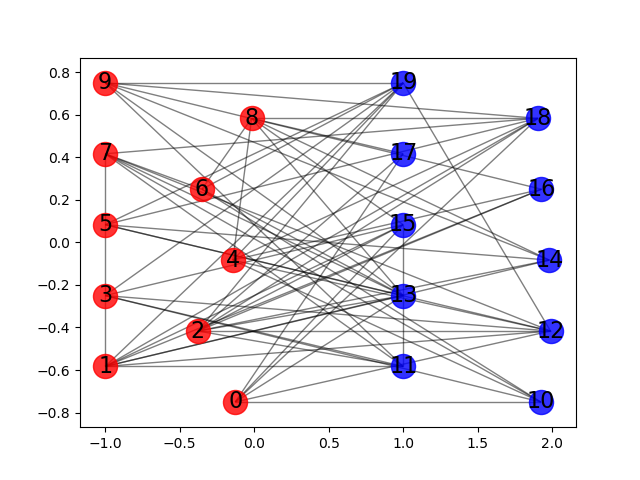
\includegraphics[width=0.85\textwidth]{Simulation_Bipartite_Example_1.png}
\caption{A visualization of the graph constructed from the previous section with 63 edges.}
\label{fig:bip_ex_1}
\end{figure}

% Add a table of data

\subsection{Analysis}
\noindent
Compare shortest paths distances data with DSD data. Analyze results.

